\documentclass[tikz,border=1pt]{standalone}
\usepackage{tikz}

\tikzset{every node/.style={shape=circle,draw = black}}
\tikzset{every edge/.style={draw = red, very thick}}
\begin{document}
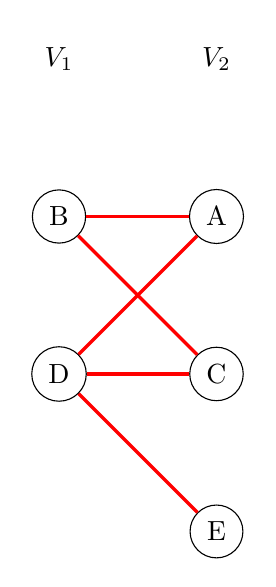
\begin{tikzpicture}[node distance = 2cm]
  \node (V1) [draw = none]{$V_1$};
  \node (V2) [draw = none,right of = V1]{$V_2$};
  \node (A) [below of = V2] {A};
  \node (B) [below of = V1] {B};
  \node (C) [below of = A] {C};
  \node (D) [below of = B] {D};
  \node (E) [below of = C] {E};

  \path (A) edge (B);
  \path (A) edge (D);

  \path (B) edge (C);

  \path (C) edge (D);

  \path (D) edge (E);
\end{tikzpicture}

\end{document}
